\documentclass[aspectratio=169,11pt]{beamer}

% =========================
% Encoding & fonts (fix UTF-8 issues in \lstlisting)
% =========================
\usepackage[utf8]{inputenc}
\usepackage[T1]{fontenc}

% Theme and appearance
\usetheme{Madrid}
\usecolortheme{seahorse}
\usefonttheme{professionalfonts}
\setbeamertemplate{navigation symbols}{}

% Packages
\usepackage{amsmath,amsthm,amssymb}
\usepackage{graphicx}
\usepackage{tikz}
\usepackage{pgfplots}
\pgfplotsset{compat=1.18}
\usepackage{algorithm,algorithmic}
\usepackage{booktabs}
\usepackage{multirow}
\usepackage{xcolor}
\usepackage{listings}
\usepackage{subcaption}
\usepackage{hyperref}

% Hyperref setup
\hypersetup{
  colorlinks=true,
  linkcolor=navyblue,
  urlcolor=navyblue,
  citecolor=navyblue
}

% Custom colors
\definecolor{navyblue}{RGB}{0,32,96}
\definecolor{crimson}{RGB}{178,34,52}
\definecolor{forest}{RGB}{34,139,34}
\definecolor{gold}{RGB}{255,215,0}
\definecolor{purple}{RGB}{128,0,128}

% Customize theme colors
\setbeamercolor{structure}{fg=navyblue}
\setbeamercolor{title}{fg=white,bg=navyblue}
\setbeamercolor{frametitle}{fg=white,bg=navyblue}
\setbeamercolor{section in toc}{fg=navyblue}

% Code listing settings
% NOTE: literate= maps problematic UTF-8 characters used inside \lstlisting.
\lstset{
    language=Python,
    basicstyle=\ttfamily\footnotesize, % smaller to reduce overfull boxes
    keywordstyle=\color{navyblue}\bfseries,
    commentstyle=\color{forest}\itshape,
    stringstyle=\color{crimson},
    numbers=left,
    numberstyle=\tiny\color{gray},
    stepnumber=1,
    tabsize=2,
    showstringspaces=false,
    breaklines=true,
    frame=single,
    rulecolor=\color{gray!30},
    keepspaces=true,
    columns=fullflexible,
    literate=
      {—}{{---}}1
      {–}{{--}}1
      {’}{{'}}1
      {‘}{{'}}1
      {“}{{"}}1
      {”}{{"}}1
      {…}{{\ldots}}1
      {×}{{$\times$}}1
      {·}{{$\cdot$}}1
      {−}{{-}}1
      {≥}{{$\ge$}}1
      {≤}{{$\le$}}1
      {≠}{{$\neq$}}1
      {→}{{$\to$}}1
      {←}{{$\leftarrow$}}1
      {°}{{$^\circ$}}1
      {²}{{\textsuperscript{2}}}1
      {³}{{\textsuperscript{3}}}1
      {α}{{$\alpha$}}1
      {β}{{$\beta$}}1
      {γ}{{$\gamma$}}1
      {λ}{{$\lambda$}}1
      {μ}{{$\mu$}}1
      {σ}{{$\sigma$}}1
      {Σ}{{$\Sigma$}}1
      {π}{{$\pi$}}1
}

% Title information
\title[Feature Engineering]{Feature Engineering \& Selection}
\subtitle{From Raw Data to ML-Ready Features}
\author[D. Ribeiro]{Diogo Ribeiro\\
\small ESMAD -- Escola Superior de Média Arte e Design\\
\small Lead Data Scientist, Mysense.ai}
\date{\today}

% Custom commands
\newcommand{\E}{\mathbb{E}}
\newcommand{\Var}{\text{Var}}
\newcommand{\Cov}{\text{Cov}}
\newcommand{\btheta}{\boldsymbol{\theta}}
\newcommand{\bx}{\mathbf{x}}
\newcommand{\by}{\mathbf{y}}
\newcommand{\bmu}{\boldsymbol{\mu}}
\newcommand{\bSigma}{\boldsymbol{\Sigma}}
\newcommand{\argmin}{\text{argmin}}
\newcommand{\argmax}{\text{argmax}}
\newcommand{\Real}{\mathbb{R}}

\begin{document}

% Title slide
\begin{frame}
\titlepage
\end{frame}

% Table of contents
\begin{frame}{Outline}
\tableofcontents
\end{frame}

\section{Introduction and Philosophy}

\begin{frame}{The Art and Science of Feature Engineering}
\begin{columns}
\begin{column}{0.6\textwidth}
\begin{quote}
\textit{"Coming up with features is difficult, time-consuming, requires expert knowledge. 'Applied machine learning' is basically feature engineering."} 
\\[0.2cm]
\hfill -- Andrew Ng
\end{quote}

\vspace{0.3cm}
\textbf{Why Features Matter:}
\begin{itemize}
\item \textcolor{crimson}{Garbage in, garbage out}: Poor features $\Rightarrow$ poor models
\item \textcolor{forest}{Domain knowledge}: Good features encode expert insights
\item \textcolor{forest}{Model performance}: Often more impact than algorithm choice
\item \textcolor{forest}{Interpretability}: Good features are meaningful to humans
\end{itemize}
\end{column}
\begin{column}{0.4\textwidth}
\begin{figure}
\centering
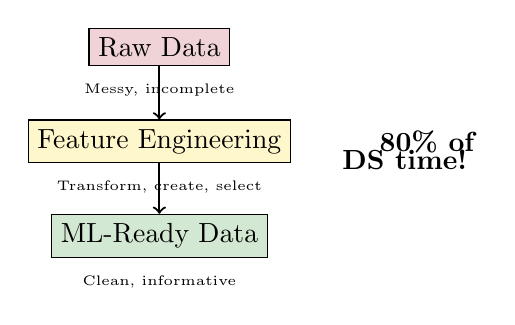
\begin{tikzpicture}[scale=0.8]
% Raw data
\node[draw, rectangle, fill=crimson!20] (raw) at (0,3) {Raw Data};
\node[below=0.1cm] at (raw.south) {\tiny Messy, incomplete};

% Feature engineering
\node[draw, rectangle, fill=gold!20] (fe) at (0,1.5) {Feature Engineering};
\node[below=0.1cm] at (fe.south) {\tiny Transform, create, select};

% ML ready
\node[draw, rectangle, fill=forest!20] (ml) at (0,0) {ML-Ready Data};
\node[below=0.1cm] at (ml.south) {\tiny Clean, informative};

% Arrows
\draw[->, thick] (raw) -- (fe);
\draw[->, thick] (fe) -- (ml);

% Side annotation
\node[right=1cm] at (fe.east) {\textbf{80\% of}};
\node[right=1cm] at (1.5,1.2) {\textbf{DS time!}};
\end{tikzpicture}
\end{figure}

\begin{alertblock}{The 80-20 Rule}
80\% of data science time is spent on data preparation and feature engineering, 20\% on modeling.
\end{alertblock}
\end{column}
\end{columns}

\vspace{0.3cm}
\textbf{This Presentation:} Systematic approach to transforming raw data into powerful, ML-ready features.
\end{frame}

\begin{frame}{Feature Engineering Pipeline Overview}
\begin{columns}
\begin{column}{0.5\textwidth}
\textbf{The Complete Pipeline:}

\begin{enumerate}
\item \textbf{Data Understanding}
   \begin{itemize}
   \item Exploratory data analysis
   \item Data quality assessment
   \item Domain knowledge integration
   \end{itemize}

\item \textbf{Cleaning \& Preprocessing}
   \begin{itemize}
   \item Missing value handling
   \item Outlier detection/treatment
   \item Data type conversions
   \end{itemize}

\item \textbf{Feature Creation}
   \begin{itemize}
   \item Transformations
   \item Interactions
   \item Domain-specific features
   \end{itemize}

\item \textbf{Feature Selection}
   \begin{itemize}
   \item Remove redundant features
   \item Statistical significance
   \item Model-based importance
   \end{itemize}
\end{enumerate}
\end{column}
\begin{column}{0.5\textwidth}
\begin{block}{Success Metrics}
\begin{itemize}
\item \textbf{Model Performance}: Accuracy, AUC, RMSE
\item \textbf{Interpretability}: Can humans understand features?
\item \textbf{Stability}: Robust to new data
\item \textbf{Efficiency}: Fast to compute and store
\end{itemize}
\end{block}

\begin{block}{Common Mistakes}
\begin{itemize}
\item \textcolor{crimson}{Data leakage}: Using future information
\item \textcolor{crimson}{Overfitting}: Too many features for sample size
\item \textcolor{crimson}{Domain ignorance}: Features that don't make sense
\item \textcolor{crimson}{Scale issues}: Forgetting normalization
\end{itemize}
\end{block}
\end{column}
\end{columns}

\begin{alertblock}{Key Principle}
Feature engineering should be \textbf{systematic}, \textbf{reproducible}, and \textbf{domain-informed}.
\end{alertblock}
\end{frame}

\section{Data Types and Transformations}

\begin{frame}{Understanding Your Data Types}
\begin{table}
\centering
\small
\begin{tabular}{p{2cm}p{3cm}p{3cm}p{3.5cm}}
\toprule
\textbf{Data Type} & \textbf{Examples} & \textbf{Challenges} & \textbf{Common Transformations} \\
\midrule
Numerical & Age, income, temperature & Skewness, outliers, scale & Log, square root, standardization \\
\midrule
Categorical & Color, country, brand & High cardinality, ordering & One-hot, label encoding, embeddings \\
\midrule
Ordinal & Education level, ratings & Preserving order & Ordinal encoding, polynomial features \\
\midrule
Temporal & Timestamps, dates & Seasonality, trends & Date parts, lags, rolling statistics \\
\midrule
Text & Reviews, descriptions & High dimensionality & TF-IDF, embeddings, sentiment \\
\midrule
Geospatial & Coordinates, addresses & Projection, distance & Distance features, clustering \\
\bottomrule
\end{tabular}
\end{table}

\begin{columns}
\begin{column}{0.5\textwidth}
\textbf{Statistical Considerations:}
\begin{itemize}
\item \textbf{Distribution shape}: Normal, skewed, multimodal?
\item \textbf{Missing patterns}: MCAR, MAR, MNAR?
\item \textbf{Correlations}: Linear, non-linear relationships?
\item \textbf{Outliers}: Measurement errors or interesting cases?
\end{itemize}
\end{column}
\begin{column}{0.5\textwidth}
\textbf{Business Considerations:}
\begin{itemize}
\item \textbf{Data availability}: What's available at prediction time?
\item \textbf{Update frequency}: How often does data change?
\item \textbf{Data quality}: How reliable are measurements?
\item \textbf{Privacy constraints}: What can we use legally?
\end{itemize}
\end{column}
\end{columns}
\end{frame}

\begin{frame}[fragile]{Numerical Feature Transformations}
\textbf{Common Issues with Numerical Features:}

\begin{columns}
\begin{column}{0.5\textwidth}
\begin{lstlisting}
import numpy as np
import pandas as pd
from scipy import stats
from sklearn.preprocessing import (
    StandardScaler, MinMaxScaler, 
    RobustScaler, PowerTransformer,
    QuantileTransformer
)

# Example: Highly skewed income data
np.random.seed(42)
income = np.random.lognormal(10, 1, 1000)
print(f"Skewness: {stats.skew(income):.2f}")
print(f"Range: [{income.min():.0f}, {income.max():.0f}]")

# Transformation strategies
transformations = {
    'log': np.log(income),
    'sqrt': np.sqrt(income),
    'box_cox': stats.boxcox(income)[0],
    'yeo_johnson': PowerTransformer().fit_transform(
        income.reshape(-1, 1)).ravel(),
    'quantile': QuantileTransformer(
        output_distribution='normal'
    ).fit_transform(income.reshape(-1, 1)).ravel()
}

# Compare skewness after transformation
for name, transformed in transformations.items():
    skew = stats.skew(transformed)
    print(f"{name:12}: skewness = {skew:5.2f}")
\end{lstlisting}
\end{column}
\begin{column}{0.5\textwidth}
\textbf{Scaling Strategies:}

\begin{itemize}
\item \textbf{StandardScaler}: $z = \frac{x - \mu}{\sigma}$
  \begin{itemize}
  \item Good for normally distributed data
  \item Sensitive to outliers
  \end{itemize}

\item \textbf{MinMaxScaler}: $x' = \frac{x - \min(x)}{\max(x) - \min(x)}$
  \begin{itemize}
  \item Bounds data to [0,1]
  \item Very sensitive to outliers
  \end{itemize}

\item \textbf{RobustScaler}: Uses median and IQR
  \begin{itemize}
  \item Robust to outliers
  \item Good for heavy-tailed distributions
  \end{itemize}
\end{itemize}

\begin{alertblock}{When to Use What?}
\textbf{Tree-based}: Often no scaling needed\\
\textbf{Linear models}: StandardScaler typically\\
\textbf{Neural networks}: MinMaxScaler or StandardScaler\\
\textbf{With outliers}: RobustScaler
\end{alertblock}
\end{column}
\end{columns}
\end{frame}

\begin{frame}[fragile]{Categorical Feature Encoding}
\textbf{The Categorical Challenge:} ML algorithms need numbers, not categories.

\begin{columns}
\begin{column}{0.55\textwidth}
\begin{lstlisting}
import pandas as pd
from sklearn.preprocessing import (
    LabelEncoder, OneHotEncoder, 
    OrdinalEncoder
)
from category_encoders import (
    TargetEncoder, BinaryEncoder,
    HashingEncoder, LeaveOneOutEncoder
)

# Sample categorical data
data = pd.DataFrame({
    'color': ['red', 'blue', 'green', 'red', 'blue'],
    'size': ['small', 'medium', 'large', 'medium', 'small'],
    'brand': ['nike', 'adidas', 'puma', 'nike', 'reebok'],
    'target': [1, 0, 1, 1, 0]
})

# 1. Label Encoding (ordinal assumption)
le = LabelEncoder()
data['color_label'] = le.fit_transform(data['color'])

# 2. One-Hot Encoding (nominal)
ohe_data = pd.get_dummies(data['color'], prefix='color')

# 3. Target Encoding (uses target info)
te = TargetEncoder()
data['brand_target_enc'] = te.fit_transform(
    data['brand'], data['target']
)

# 4. Binary Encoding (for high cardinality)
be = BinaryEncoder()
brand_binary = be.fit_transform(data['brand'])

# 5. Hashing (for very high cardinality)
he = HashingEncoder(n_components=3)
brand_hash = he.fit_transform(data['brand'])

print("Encoding comparison:")
print("Original brands:", data['brand'].unique())
print("Label encoded:", data['color_label'].unique())
print("Target encoded mean:", data.groupby('brand')['brand_target_enc'].mean())
\end{lstlisting}
\end{column}
\begin{column}{0.45\textwidth}
\textbf{Encoding Strategy Guide:}

\begin{table}
\centering
\tiny
\begin{tabular}{p{2cm}p{1.5cm}p{1.5cm}}
\toprule
\textbf{Method} & \textbf{Cardinality} & \textbf{Best For} \\
\midrule
Label & Any & Ordinal data \\
One-Hot & Low ($<10$) & Nominal data \\
Target & Medium & High predictive power \\
Binary & High ($<1000$) & Memory efficient \\
Hashing & Very High & Streaming data \\
\bottomrule
\end{tabular}
\end{table}

\vspace{0.3cm}
\textbf{Advanced Techniques:}
\begin{itemize}
\item \textbf{Embeddings}: Learn dense representations
\item \textbf{Frequency encoding}: Replace with counts
\item \textbf{Leave-one-out}: Avoid target leakage
\item \textbf{CatBoost encoding}: Ordered target statistics
\end{itemize}

\begin{alertblock}{Pitfall Warning}
\textcolor{crimson}{\textbf{Target leakage}} in target encoding! Always use cross-validation or leave-one-out.
\end{alertblock}
\end{column}
\end{columns}
\end{frame}

\begin{frame}[fragile]{Temporal Feature Engineering}
\textbf{Time Series Features:} Extract meaningful patterns from timestamps.

\begin{columns}
\begin{column}{0.55\textwidth}
\begin{lstlisting}
import pandas as pd
import numpy as np
from datetime import datetime, timedelta

# Sample time series data
dates = pd.date_range(start='2020-01-01', end='2023-12-31', freq='D')
np.random.seed(42)
sales = 100 + 10*np.sin(2*np.pi*np.arange(len(dates))/365.25) + \
        5*np.random.randn(len(dates))

df = pd.DataFrame({'date': dates, 'sales': sales})
df['date'] = pd.to_datetime(df['date'])

# Basic temporal features
df['year'] = df['date'].dt.year
df['month'] = df['date'].dt.month
df['day'] = df['date'].dt.day
df['dayofweek'] = df['date'].dt.dayofweek
df['quarter'] = df['date'].dt.quarter
df['is_weekend'] = df['dayofweek'].isin([5, 6])

# Cyclical encoding (preserves distance)
df['month_sin'] = np.sin(2 * np.pi * df['month'] / 12)
df['month_cos'] = np.cos(2 * np.pi * df['month'] / 12)

# Rolling statistics
df['sales_7d_mean'] = df['sales'].rolling(7).mean()
df['sales_7d_std'] = df['sales'].rolling(7).std()
df['sales_30d_mean'] = df['sales'].rolling(30).mean()

# Lag features
df['sales_lag1'] = df['sales'].shift(1)
df['sales_lag7'] = df['sales'].shift(7)
df['sales_lag365'] = df['sales'].shift(365)

# Differences
df['sales_diff1'] = df['sales'].diff(1)
df['sales_diff7'] = df['sales'].diff(7)

# Time since event features
black_friday = pd.to_datetime(['2020-11-27', '2021-11-26', 
                              '2022-11-25', '2023-11-24'])
df['days_since_black_friday'] = df['date'].apply(
    lambda x: min([(x - bf).days for bf in black_friday if x >= bf] + [999])
)

print("Temporal features created:")
print(df.columns.tolist())
\end{lstlisting}
\end{column}
\begin{column}{0.45\textwidth}
\textbf{Temporal Feature Categories:}

\begin{itemize}
\item \textbf{Date Parts}: Year, month, day, hour
\item \textbf{Cyclical}: Sin/cos encoding for seasonality
\item \textbf{Rolling Statistics}: Moving averages, std
\item \textbf{Lags}: Historical values
\item \textbf{Differences}: Trend indicators
\item \textbf{Event-based}: Time since/until events
\end{itemize}

\vspace{0.3cm}
\begin{block}{Holiday Features}
\begin{itemize}
\item Is holiday? (binary)
\item Days until next holiday
\item Holiday type (religious, national, etc.)
\item Regional holidays
\end{itemize}
\end{block}

\begin{alertblock}{Data Leakage Alert}
Never use future information! Always ensure lag features use only past data at prediction time.
\end{alertblock}
\end{column}
\end{columns}
\end{frame}

\section{Advanced Feature Creation}

\begin{frame}[fragile]{Polynomial and Interaction Features}
\textbf{Capturing Non-linear Relationships:}

\begin{columns}
\begin{column}{0.5\textwidth}
\begin{lstlisting}
import numpy as np
import pandas as pd
from sklearn.preprocessing import PolynomialFeatures
from sklearn.model_selection import cross_val_score
from sklearn.linear_model import LinearRegression
from sklearn.pipeline import Pipeline

# Generate sample data with interactions
np.random.seed(42)
n_samples = 1000
X1 = np.random.randn(n_samples)
X2 = np.random.randn(n_samples)
X3 = np.random.randn(n_samples)

# True relationship with interactions
y = (2*X1 + 3*X2 + 1.5*X1*X2 + 
     0.5*X1**2 + np.random.randn(n_samples)*0.1)

df = pd.DataFrame({'X1': X1, 'X2': X2, 'X3': X3, 'y': y})

# Manual interaction features
df['X1_X2'] = df['X1'] * df['X2']
df['X1_squared'] = df['X1'] ** 2
df['X2_squared'] = df['X2'] ** 2

# Automatic polynomial features
poly = PolynomialFeatures(degree=2, 
                         include_bias=False,
                         interaction_only=False)
X_poly = poly.fit_transform(df[['X1', 'X2', 'X3']])
feature_names = poly.get_feature_names_out(['X1', 'X2', 'X3'])

print("Original features:", ['X1', 'X2', 'X3'])
print("Polynomial features:", feature_names)

# Compare model performance
X_original = df[['X1', 'X2', 'X3']]
X_manual = df[['X1', 'X2', 'X3', 'X1_X2', 'X1_squared', 'X2_squared']]

models = {
    'Linear': X_original,
    'Manual Interactions': X_manual,
    'Polynomial': X_poly
}

for name, X in models.items():
    score = cross_val_score(LinearRegression(), X, df['y'], cv=5).mean()
    print(f"{name}: R^2 = {score:.4f}")
\end{lstlisting}
\end{column}
\begin{column}{0.5\textwidth}
\textbf{When to Use Polynomial Features:}

\begin{itemize}
\item \textcolor{forest}{Linear models}: Add non-linearity
\item \textcolor{forest}{Known relationships}: Domain knowledge suggests interactions
\item \textcolor{crimson}{High-dimensional data}: Curse of dimensionality
\item \textcolor{crimson}{Tree-based models}: Usually unnecessary
\end{itemize}

\vspace{0.3cm}
\textbf{Feature Explosion Problem:}
\begin{align}
\text{Degree 2:} \quad &\binom{d+2}{2} \text{ features}\\
\text{Degree 3:} \quad &\binom{d+3}{3} \text{ features}
\end{align}

For $d=10$ features:
\begin{itemize}
\item Degree 2: 66 features
\item Degree 3: 286 features
\end{itemize}

\begin{block}{Practical Strategy}
\begin{enumerate}
\item Start with domain-knowledge interactions
\item Use feature selection to prune
\item Consider regularization (Ridge, Lasso)
\item Monitor for overfitting
\end{enumerate}
\end{block}
\end{column}
\end{columns}
\end{frame}

\begin{frame}[fragile]{Domain-Specific Feature Engineering}
\textbf{Case Study: E-commerce Customer Features}

\begin{columns}
\begin{column}{0.55\textwidth}
\begin{lstlisting}
import pandas as pd
import numpy as np
from datetime import datetime, timedelta

# Sample e-commerce transaction data
np.random.seed(42)
transactions = pd.DataFrame({
    'customer_id': np.repeat(range(1000), 10),
    'transaction_date': pd.to_datetime('2023-01-01') + 
                       pd.to_timedelta(np.random.randint(0, 365, 10000), unit='D'),
    'amount': np.random.exponential(50, 10000),
    'product_category': np.random.choice(['electronics', 'clothing', 'books', 'home'], 10000),
    'is_returned': np.random.binomial(1, 0.1, 10000)
})

# Feature engineering at customer level
def create_customer_features(df, analysis_date='2023-12-31'):
    analysis_date = pd.to_datetime(analysis_date)
    
    customer_features = df.groupby('customer_id').agg({
        # Recency features
        'transaction_date': [
            lambda x: (analysis_date - x.max()).days,  # days_since_last_purchase
            lambda x: (analysis_date - x.min()).days,  # customer_lifetime_days
            'count'  # transaction_frequency
        ],
        # Monetary features
        'amount': ['sum', 'mean', 'std', 'max', 'min'],
        # Return behavior
        'is_returned': ['sum', 'mean']
    }).round(2)
    
    # Flatten column names
    customer_features.columns = ['_'.join(col).strip() for col in customer_features.columns]
    customer_features = customer_features.reset_index()
    
    # Additional computed features
    customer_features['avg_days_between_purchases'] = (
        customer_features['transaction_date_<lambda_1>'] / 
        customer_features['transaction_date_count']
    )
    
    customer_features['total_returned_amount'] = (
        customer_features['is_returned_sum'] * customer_features['amount_mean']
    )
    
    # RFM Score (Recency, Frequency, Monetary)
    customer_features['rfm_score'] = (
        pd.qcut(customer_features['transaction_date_<lambda_0>'], 5, labels=False) +
        pd.qcut(customer_features['transaction_date_count'], 5, labels=False) +
        pd.qcut(customer_features['amount_sum'], 5, labels=False)
    )
    
    return customer_features

customer_df = create_customer_features(transactions)
print("Customer features shape:", customer_df.shape)
print("\nSample features:")
print(customer_df.head())
\end{lstlisting}
\end{column}
\begin{column}{0.45\textwidth}
\textbf{Domain-Specific Feature Types:}

\begin{itemize}
\item \textbf{RFM Analysis}:
  \begin{itemize}
  \item Recency: Days since last purchase
  \item Frequency: Number of transactions
  \item Monetary: Total/average spend
  \end{itemize}

\item \textbf{Behavioral Patterns}:
  \begin{itemize}
  \item Purchase seasonality
  \item Category preferences
  \item Return behavior
  \item Price sensitivity
  \end{itemize}

\item \textbf{Trend Features}:
  \begin{itemize}
  \item Spending trend (increasing/decreasing)
  \item Category shift patterns
  \item Engagement trends
  \end{itemize}
\end{itemize}

\begin{block}{Industry Examples}
\textbf{Finance}: Credit utilization, payment history\\
\textbf{Healthcare}: Vital sign trends, medication adherence\\
\textbf{Marketing}: CTR, conversion funnels\\
\textbf{Manufacturing}: Sensor patterns, maintenance cycles
\end{block}
\end{column}
\end{columns}

\textbf{Key Insight:} The best features often come from deep domain understanding, not just statistical techniques.
\end{frame}

\section{Dimensionality Reduction}

\begin{frame}{The Curse of Dimensionality}
\begin{columns}
\begin{column}{0.5\textwidth}
\textbf{Why High Dimensions Are Problematic:}

\begin{itemize}
\item \textbf{Sparsity}: Data points become sparse in high-D space
\item \textbf{Distance concentration}: All points equidistant
\item \textbf{Overfitting}: More parameters than samples
\item \textbf{Computational cost}: $O(d^k)$ complexity
\item \textbf{Visualization}: Impossible to plot $>3$D
\end{itemize}

\vspace{0.3cm}
\textbf{Mathematical Intuition:}
Volume of unit hypersphere in $d$ dimensions:
\[V_d = \frac{\pi^{d/2}}{\Gamma(d/2 + 1)}\]

As $d \to \infty$, $V_d \to 0$ (volume concentrates at surface)
\end{column}
\begin{column}{0.5\textwidth}
\begin{figure}
\centering
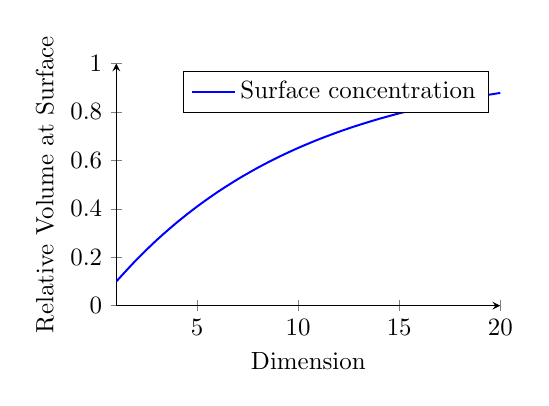
\begin{tikzpicture}[scale=0.9]
\begin{axis}[
    xlabel={Dimension},
    ylabel={Relative Volume at Surface},
    width=7cm,
    height=5cm,
    axis lines=left,
    xmin=1, xmax=20,
    ymin=0, ymax=1,
    legend pos=north east
]
\addplot[domain=1:20, samples=20, smooth, thick, blue] {1 - (0.9)^x};
\addlegendentry{Surface concentration}
\end{axis}
\end{tikzpicture}
\end{figure}

\begin{alertblock}{The $d \gg n$ Problem}
When dimensions exceed samples:
\begin{itemize}
\item Perfect separation possible
\item No generalization
\item Regularization essential
\end{itemize}
\end{alertblock}
\end{column}
\end{columns}

\textbf{Solution:} Reduce dimensionality while preserving important information.
\end{frame}

\begin{frame}[fragile]{Principal Component Analysis (PCA)}
\textbf{Goal:} Find linear combinations of features that maximize variance.

\begin{columns}
\begin{column}{0.5\textwidth}
\textbf{Mathematical Formulation:}
\begin{align}
\text{Maximize:} \quad &\text{Var}(\mathbf{w}^T \mathbf{X})\\
\text{Subject to:} \quad &\|\mathbf{w}\|^2 = 1
\end{align}

\textbf{Solution:} Eigenvectors of covariance matrix
\[\mathbf{C} = \frac{1}{n-1}\mathbf{X}^T\mathbf{X}\]

\textbf{Principal Components:}
\[\mathbf{PC}_i = \mathbf{X} \mathbf{v}_i\]
where $\mathbf{v}_i$ are eigenvectors ordered by eigenvalue magnitude.

\vspace{0.3cm}
\textbf{Variance Explained:}
\[\text{Proportion}_i = \frac{\lambda_i}{\sum_{j=1}^d \lambda_j}\]
\end{column}
\begin{column}{0.5\textwidth}
\begin{lstlisting}
import numpy as np
import matplotlib.pyplot as plt
from sklearn.decomposition import PCA
from sklearn.datasets import load_breast_cancer
from sklearn.preprocessing import StandardScaler

# Load high-dimensional dataset
data = load_breast_cancer()
X, y = data.data, data.target

print(f"Original dimensions: {X.shape}")

# Standardize features (crucial for PCA)
scaler = StandardScaler()
X_scaled = scaler.fit_transform(X)

# Apply PCA
pca = PCA()
X_pca = pca.fit_transform(X_scaled)

# Analyze variance explained
cumsum_var = np.cumsum(pca.explained_variance_ratio_)
n_components_95 = np.argmax(cumsum_var >= 0.95) + 1

print(f"Components for 95% variance: {n_components_95}")
print(f"Original features: {X.shape[1]}")
print(f"Dimension reduction: {X.shape[1]/n_components_95:.1f}x")

# Plot variance explained
plt.figure(figsize=(10, 4))
plt.subplot(1, 2, 1)
plt.plot(pca.explained_variance_ratio_[:20], 'o-')
plt.xlabel('Component')
plt.ylabel('Variance Explained')
plt.title('Individual Components')

plt.subplot(1, 2, 2)
plt.plot(cumsum_var[:20], 'o-')
plt.axhline(y=0.95, linestyle='--')
plt.xlabel('Number of Components')
plt.ylabel('Cumulative Variance')
plt.title('Cumulative Variance')
plt.tight_layout()
\end{lstlisting}
\end{column}
\end{columns}
\end{frame}

\begin{frame}[fragile]{Advanced Dimensionality Reduction Techniques}
\textbf{Non-linear Methods for Complex Data:}

\begin{columns}
\begin{column}{0.55\textwidth}
\begin{lstlisting}
import numpy as np
from sklearn.manifold import TSNE
from umap import UMAP
from sklearn.decomposition import KernelPCA
from sklearn.datasets import make_swiss_roll

# Generate non-linear data
X, color = make_swiss_roll(n_samples=1000, noise=0.1)

# 1. Kernel PCA (non-linear PCA)
kpca_rbf = KernelPCA(n_components=2, kernel='rbf', gamma=0.1)
X_kpca = kpca_rbf.fit_transform(X)

# 2. t-SNE (preserves local structure)
tsne = TSNE(n_components=2, perplexity=30, random_state=42)
X_tsne = tsne.fit_transform(X)

# 3. UMAP (preserves global and local structure)
umap = UMAP(n_components=2, random_state=42)
X_umap = umap.fit_transform(X)

# Visualization comparison
import matplotlib.pyplot as plt

fig, axes = plt.subplots(2, 2, figsize=(12, 10))

# Original 3D data (first 2 dimensions)
axes[0,0].scatter(X[:, 0], X[:, 1], c=color)
axes[0,0].set_title('Original Data (2D projection)')

# Kernel PCA
axes[0,1].scatter(X_kpca[:, 0], X_kpca[:, 1], c=color)
axes[0,1].set_title('Kernel PCA')

# t-SNE
axes[1,0].scatter(X_tsne[:, 0], X_tsne[:, 1], c=color)
axes[1,0].set_title('t-SNE')

# UMAP
axes[1,1].scatter(X_umap[:, 0], X_umap[:, 1], c=color)
axes[1,1].set_title('UMAP')

plt.tight_layout()
print("Dimensionality reduction comparison complete")

# Performance characteristics
methods = {
    'PCA': 'Linear, fast, interpretable',
    'Kernel PCA': 'Non-linear, medium speed, less interpretable',
    't-SNE': 'Non-linear, slow, great for visualization',
    'UMAP': 'Non-linear, fast, preserves global structure'
}
for method, description in methods.items():
    print(f"{method:10}: {description}")
\end{lstlisting}
\end{column}
\begin{column}{0.45\textwidth}
\textbf{Method Comparison:}

\begin{table}
\centering
\tiny
\begin{tabular}{p{1.5cm}p{1cm}p{1cm}p{1.5cm}}
\toprule
\textbf{Method} & \textbf{Linear?} & \textbf{Speed} & \textbf{Best For} \\
\midrule
PCA & Yes & Fast & Feature reduction \\
Kernel PCA & No & Medium & Non-linear patterns \\
t-SNE & No & Slow & Visualization \\
UMAP & No & Fast & General purpose \\
LLE & No & Medium & Manifold learning \\
Isomap & No & Medium & Geodesic distances \\
\bottomrule
\end{tabular}
\end{table}

\vspace{0.3cm}
\textbf{Choosing the Right Method:}
\begin{itemize}
\item \textbf{Linear relationships}: PCA
\item \textbf{Interpretation needed}: PCA, Factor Analysis
\item \textbf{Visualization}: t-SNE, UMAP
\item \textbf{Manifold structure}: UMAP, LLE, Isomap
\item \textbf{Speed critical}: PCA, UMAP
\end{itemize}

\begin{alertblock}{Common Pitfalls}
\begin{itemize}
\item t-SNE: Don't interpret distances between clusters
\item UMAP: Hyperparameters matter a lot
\item All: Validate on downstream task performance
\end{itemize}
\end{alertblock}
\end{column}
\end{columns}
\end{frame}

\section{Feature Selection Methods}

\begin{frame}{Feature Selection: Why and When}
\begin{columns}
\begin{column}{0.5\textwidth}
\textbf{Why Remove Features?}

\begin{itemize}
\item \textcolor{crimson}{\textbf{Overfitting}}: Too many features relative to samples
\item \textcolor{crimson}{\textbf{Noise}}: Irrelevant features hurt performance
\item \textcolor{crimson}{\textbf{Multicollinearity}}: Redundant information
\item \textcolor{crimson}{\textbf{Computational cost}}: Storage and processing
\item \textcolor{crimson}{\textbf{Interpretability}}: Simpler models are easier to understand
\end{itemize}

\vspace{0.3cm}
\textbf{The Bias-Variance Perspective:}
\begin{align}
\text{Fewer features} &\Rightarrow \text{Higher bias, Lower variance}\\
\text{More features} &\Rightarrow \text{Lower bias, Higher variance}
\end{align}

\textbf{Goal:} Find the sweet spot that minimizes total error.
\end{column}
\begin{column}{0.5\textwidth}
\begin{figure}
\centering
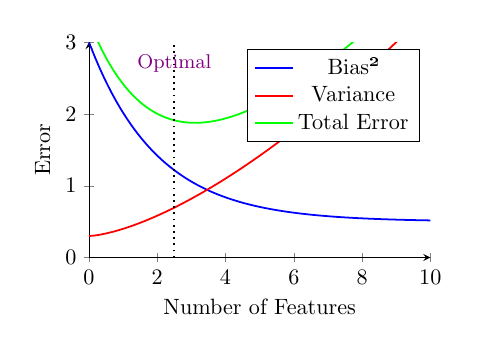
\begin{tikzpicture}[scale=0.8]
\begin{axis}[
    xlabel={Number of Features},
    ylabel={Error},
    width=7cm,
    height=5cm,
    axis lines=left,
    xmin=0, xmax=10,
    ymin=0, ymax=3,
    legend pos=north east
]
\addplot[domain=0:10, samples=100, smooth, thick, blue] {2.5*exp(-x/2) + 0.5};
\addlegendentry{Bias²}
\addplot[domain=0:10, samples=100, smooth, thick, red] {0.1*x^1.5 + 0.3};
\addlegendentry{Variance}
\addplot[domain=0:10, samples=100, smooth, thick, green] {2.5*exp(-x/2) + 0.1*x^1.5 + 0.8};
\addlegendentry{Total Error}
\draw[dotted, thick] (axis cs:2.5,0) -- (axis cs:2.5,3);
\node at (axis cs:2.5,2.7) {\textcolor{purple}{\small Optimal}};
\end{axis}
\end{tikzpicture}
\end{figure}

\begin{block}{When to Apply Feature Selection}
\begin{itemize}
\item High-dimensional data ($p \gg n$)
\item Noisy or redundant features
\item Interpretability requirements
\item Computational constraints
\item Model deployment concerns
\end{itemize}
\end{block}
\end{column}
\end{columns}

\textbf{Three Main Approaches:} Filter, Wrapper, and Embedded methods.
\end{frame}

\begin{frame}[fragile]{Filter Methods: Statistical Feature Selection}
\textbf{Idea:} Rank features by statistical measures, independent of the learning algorithm.

\begin{columns}
\begin{column}{0.55\textwidth}
\begin{lstlisting}
import numpy as np
import pandas as pd
from sklearn.datasets import make_classification
from sklearn.feature_selection import (
    SelectKBest, f_classif, chi2, 
    mutual_info_classif,
    VarianceThreshold,
    SelectPercentile
)
from sklearn.preprocessing import StandardScaler
from scipy.stats import pearsonr

# Generate sample data with irrelevant features
X, y = make_classification(
    n_samples=1000, n_features=20, 
    n_informative=5, n_redundant=3,
    n_clusters_per_class=1, random_state=42
)

feature_names = [f'feature_{i}' for i in range(X.shape[1])]
df = pd.DataFrame(X, columns=feature_names)
df['target'] = y

print(f"Original features: {X.shape[1]}")

# 1. Variance Threshold (remove low-variance features)
variance_selector = VarianceThreshold(threshold=0.1)
X_variance = variance_selector.fit_transform(X)
print(f"After variance threshold: {X_variance.shape[1]}")

# 2. Univariate statistical tests
# For classification: f_classif, chi2, mutual_info_classif
k_best_f = SelectKBest(score_func=f_classif, k=10)
X_f_test = k_best_f.fit_transform(X, y)
f_scores = k_best_f.scores_
f_pvalues = k_best_f.pvalues_

print(f"After F-test (k=10): {X_f_test.shape[1]}")
print(f"F-test scores range: [{f_scores.min():.2f}, {f_scores.max():.2f}]")

# 3. Mutual Information
mi_selector = SelectKBest(score_func=mutual_info_classif, k=10)
X_mi = mi_selector.fit_transform(X, y)
mi_scores = mi_selector.scores_

print(f"MI scores range: [{mi_scores.min():.3f}, {mi_scores.max():.3f}]")

# 4. Correlation-based selection
def correlation_selector(X, y, threshold=0.1):
    """Select features with high correlation to target"""
    correlations = []
    for i in range(X.shape[1]):
        corr, _ = pearsonr(X[:, i], y)
        correlations.append(abs(corr))
    selected_idx = [i for i, corr in enumerate(correlations) if corr > threshold]
    return X[:, selected_idx], selected_idx

X_corr, corr_idx = correlation_selector(X, y, threshold=0.2)
print(f"After correlation selection: {X_corr.shape[1]}")

# Feature ranking comparison
feature_rankings = pd.DataFrame({
    'feature': feature_names,
    'f_score': f_scores,
    'mi_score': mi_scores,
    'f_rank': (-f_scores).argsort().argsort() + 1,
    'mi_rank': (-mi_scores).argsort().argsort() + 1
})

print("\nTop 5 features by F-test:")
print(feature_rankings.nsmallest(5, 'f_rank')[['feature', 'f_score', 'f_rank']])
\end{lstlisting}
\end{column}
\begin{column}{0.45\textwidth}
\textbf{Filter Method Types:}

\begin{itemize}
\item \textbf{Variance Threshold}:
  \begin{itemize}
  \item Remove constant/quasi-constant features
  \item Fast, unsupervised
  \end{itemize}

\item \textbf{Statistical Tests}:
  \begin{itemize}
  \item F-test: Linear relationships
  \item Chi-square: Categorical features
  \item Mutual Information: Non-linear relationships
  \end{itemize}

\item \textbf{Correlation Methods}:
  \begin{itemize}
  \item Pearson: Linear correlation
  \item Spearman: Monotonic relationships
  \item Distance correlation: General dependence
  \end{itemize}
\end{itemize}

\begin{block}{Pros and Cons}
\textbf{Pros:}
\begin{itemize}
\item Fast and scalable
\item Model-agnostic
\item Good for initial screening
\end{itemize}

\textbf{Cons:}
\begin{itemize}
\item Ignores feature interactions
\item May miss non-linear relationships
\item No consideration of target model
\end{itemize}
\end{block}
\end{column}
\end{columns}
\end{frame}

\begin{frame}[fragile]{Wrapper Methods: Model-Based Selection}
\textbf{Idea:} Use the target model's performance to evaluate feature subsets.

\begin{columns}
\begin{column}{0.55\textwidth}
\begin{lstlisting}
import numpy as np
from sklearn.model_selection import cross_val_score
from sklearn.ensemble import RandomForestClassifier
from sklearn.feature_selection import (
    RFE, RFECV, SequentialFeatureSelector
)
from sklearn.linear_model import LogisticRegression
from sklearn.datasets import make_classification

# Generate data
X, y = make_classification(
    n_samples=500, n_features=15, 
    n_informative=5, n_redundant=3,
    random_state=42
)

print(f"Original features: {X.shape[1]}")

# 1. Recursive Feature Elimination (RFE)
estimator = LogisticRegression(random_state=42, max_iter=2000)
rfe = RFE(estimator=estimator, n_features_to_select=5)
X_rfe = rfe.fit_transform(X, y)

print(f"RFE selected features: {X_rfe.shape[1]}")
print(f"Selected feature mask: {rfe.support_}")
print(f"Feature ranking: {rfe.ranking_}")

# 2. RFE with Cross-Validation (automatic selection)
rfecv = RFECV(
    estimator=estimator, 
    step=1, 
    cv=5, 
    scoring='accuracy',
    min_features_to_select=2
)
X_rfecv = rfecv.fit_transform(X, y)

print(f"RFECV optimal features: {X_rfecv.shape[1]}")

# 3. Sequential Feature Selection
# Forward selection
sfs_forward = SequentialFeatureSelector(
    estimator, 
    n_features_to_select=5,
    direction='forward',
    cv=3
)
X_sfs_forward = sfs_forward.fit_transform(X, y)

# Backward elimination
sfs_backward = SequentialFeatureSelector(
    estimator,
    n_features_to_select=5, 
    direction='backward',
    cv=3
)
X_sfs_backward = sfs_backward.fit_transform(X, y)

print(f"Forward selection: {X_sfs_forward.shape[1]} features")
print(f"Backward elimination: {X_sfs_backward.shape[1]} features")

# Performance comparison
methods = {
    'Original': X,
    'RFE': X_rfe,
    'RFECV': X_rfecv,
    'Forward': X_sfs_forward,
    'Backward': X_sfs_backward
}

print("\nPerformance comparison:")
for name, X_selected in methods.items():
    score = cross_val_score(
        LogisticRegression(random_state=42, max_iter=2000), 
        X_selected, y, cv=5
    ).mean()
    print(f"{name:10}: {score:.4f} ({X_selected.shape[1]} features)")
\end{lstlisting}
\end{column}
\begin{column}{0.45\textwidth}
\textbf{Wrapper Method Types:}

\begin{itemize}
\item \textbf{Forward Selection}:
  \begin{itemize}
  \item Start empty, add best feature iteratively
  \item Fast, but can get stuck in local optima
  \end{itemize}

\item \textbf{Backward Elimination}:
  \begin{itemize}
  \item Start with all, remove worst iteratively
  \item More thorough, computationally expensive
  \end{itemize}

\item \textbf{Recursive Feature Elimination}:
  \begin{itemize}
  \item Use model's feature importance
  \item Remove least important iteratively
  \end{itemize}
\end{itemize}

\vspace{0.3cm}
\textbf{Search Strategies:}
\begin{itemize}
\item Exhaustive (intractable for large $p$)
\item Greedy (forward/backward)
\item Floating (can add/remove features)
\item Genetic algorithms
\item Simulated annealing
\end{itemize}

\begin{alertblock}{Computational Cost}
Wrapper methods are expensive: $O(2^p)$ for exhaustive search, $O(p^2)$ for greedy.
\end{alertblock}
\end{column}
\end{columns}
\end{frame}

\begin{frame}[fragile]{Embedded Methods: Built-in Feature Selection}
\textbf{Idea:} Feature selection is integrated into the model training process.

\begin{columns}
\begin{column}{0.55\textwidth}
\begin{lstlisting}
import numpy as np
import matplotlib.pyplot as plt
from sklearn.datasets import make_regression
from sklearn.linear_model import Lasso, Ridge, ElasticNet
from sklearn.ensemble import RandomForestRegressor
from sklearn.feature_selection import SelectFromModel
from sklearn.model_selection import cross_val_score

# Generate regression data with some irrelevant features
X, y = make_regression(
    n_samples=200, n_features=20, 
    n_informative=5, noise=10,
    random_state=42
)

print(f"Original features: {X.shape[1]}")

# 1. L1 Regularization (Lasso) - automatic feature selection
alphas = np.logspace(-4, 1, 50)
lasso_scores = []
n_features_selected = []

for alpha in alphas:
    lasso = Lasso(alpha=alpha, max_iter=2000)
    score = cross_val_score(lasso, X, y, cv=5).mean()
    lasso_scores.append(score)
    lasso.fit(X, y)
    n_selected = np.sum(lasso.coef_ != 0)
    n_features_selected.append(n_selected)

# Find best alpha
best_idx = np.argmax(lasso_scores)
best_alpha = alphas[best_idx]
print(f"Best Lasso alpha: {best_alpha:.4f}")
print(f"Features selected: {n_features_selected[best_idx]}")

# 2. Tree-based feature importance
rf = RandomForestRegressor(n_estimators=100, random_state=42)
rf.fit(X, y)
importances = rf.feature_importances_

# Select features using importance threshold
selector = SelectFromModel(rf, threshold='mean')
X_rf_selected = selector.fit_transform(X, y)
print(f"RF selected features: {X_rf_selected.shape[1]}")

# 3. ElasticNet (combines L1 and L2)
elastic = ElasticNet(alpha=0.1, l1_ratio=0.7, random_state=42)
elastic.fit(X, y)
elastic_selected = np.sum(elastic.coef_ != 0)
print(f"ElasticNet selected features: {elastic_selected}")

# Visualization (no explicit colors to keep style neutral)
fig, axes = plt.subplots(1, 3, figsize=(15, 4))

# Lasso path
axes[0].semilogx(alphas, lasso_scores, label='CV Score')
axes[0].axvline(best_alpha, linestyle='--', label='Best alpha')
axes[0].set_xlabel('Alpha')
axes[0].set_ylabel('CV Score')
axes[0].set_title('Lasso Regularization Path')
axes[0].legend()

# Feature selection vs alpha
axes[1].semilogx(alphas, n_features_selected)
axes[1].axvline(best_alpha, linestyle='--')
axes[1].set_xlabel('Alpha')
axes[1].set_ylabel('Features Selected')
axes[1].set_title('Features vs Regularization')

# Feature importance
feature_idx = np.arange(X.shape[1])
axes[2].bar(feature_idx, importances)
axes[2].axhline(importances.mean(), linestyle='--', label='Mean')
axes[2].set_xlabel('Feature Index')
axes[2].set_ylabel('Importance')
axes[2].set_title('Random Forest Feature Importance')
axes[2].legend()

plt.tight_layout()
\end{lstlisting}
\end{column}
\begin{column}{0.45\textwidth}
\textbf{Embedded Method Types:}

\begin{itemize}
\item \textbf{L1 Regularization (Lasso)}:
  \begin{itemize}
  \item Penalty: $\lambda \sum_j |\beta_j|$
  \item Sets coefficients exactly to zero
  \item Automatic feature selection
  \end{itemize}

\item \textbf{Tree-based Importance}:
  \begin{itemize}
  \item Random Forest, Gradient Boosting
  \item Based on split improvement
  \item Handles interactions naturally
  \end{itemize}

\item \textbf{ElasticNet}:
  \begin{itemize}
  \item Combines L1 and L2 penalties
  \item Groups correlated features
  \item More stable than pure Lasso
  \end{itemize}
\end{itemize}

\vspace{0.3cm}
\begin{block}{Advantages}
\begin{itemize}
\item Efficient (single training run)
\item Model-specific feature importance
\item Handles feature interactions
\item Less prone to overfitting
\end{itemize}
\end{block}

\begin{alertblock}{Model-Specific Results}
Feature importance depends on the model used. Always validate on your target algorithm.
\end{alertblock}
\end{column}
\end{columns}
\end{frame}

\section{Practical Considerations and Best Practices}

\begin{frame}{Data Leakage: The Silent Killer}
\begin{columns}
\begin{column}{0.5\textwidth}
\textbf{What is Data Leakage?}
Information from the future or target variable inadvertently included in features.

\vspace{0.3cm}
\textbf{Types of Leakage:}

\begin{itemize}
\item \textcolor{crimson}{\textbf{Temporal leakage}}: Using future information
\item \textcolor{crimson}{\textbf{Target leakage}}: Features that contain target info
\item \textcolor{crimson}{\textbf{Train-test leakage}}: Data preprocessing on full dataset
\end{itemize}

\vspace{0.3cm}
\textbf{Common Examples:}
\begin{itemize}
\item Credit scoring using payment history after loan decision
\item Medical diagnosis using treatment information
\item Sales prediction using quarterly totals
\item Stock prediction using next-day prices
\end{itemize}
\end{column}
\begin{column}{0.5\textwidth}
\textbf{Preventing Leakage:}

\begin{enumerate}
\item \textbf{Time-aware splits}:
   \begin{itemize}
   \item Train on past, test on future
   \item No random shuffling for time series
   \end{itemize}

\item \textbf{Proper preprocessing}:
   \begin{itemize}
   \item Fit transformers only on training data
   \item Apply to test data, don't refit
   \end{itemize}

\item \textbf{Domain knowledge}:
   \begin{itemize}
   \item What information is available when?
   \item Business process understanding
   \end{itemize}

\item \textbf{Feature audit}:
   \begin{itemize}
   \item Check correlations with target
   \item Validate with domain experts
   \end{itemize}
\end{enumerate}

\begin{alertblock}{Golden Rule}
Only use information that would be available at prediction time in the real world.
\end{alertblock}
\end{column}
\end{columns}
\end{frame}

\begin{frame}[fragile]{Pipeline Design and Reproducibility}
\textbf{Best Practice:} Use sklearn pipelines for reproducible feature engineering.

\begin{columns}
\begin{column}{0.6\textwidth}
\begin{lstlisting}
import pandas as pd
import numpy as np
from sklearn.pipeline import Pipeline
from sklearn.compose import ColumnTransformer
from sklearn.preprocessing import (
    StandardScaler, OneHotEncoder, 
    FunctionTransformer
)
from sklearn.feature_selection import SelectKBest, f_regression
from sklearn.ensemble import RandomForestRegressor
from sklearn.model_selection import cross_val_score

# Sample mixed-type dataset
np.random.seed(42)
data = pd.DataFrame({
    'numeric1': np.random.randn(1000),
    'numeric2': np.random.exponential(2, 1000),
    'category1': np.random.choice(['A', 'B', 'C'], 1000),
    'category2': np.random.choice(['X', 'Y'], 1000),
    'date': pd.date_range('2020-01-01', periods=1000, freq='D')
})

# Create target with some relationship to features
data['target'] = (2 * data['numeric1'] + 
                 np.where(data['category1'] == 'A', 5, 0) +
                 np.random.randn(1000))

# Custom date feature extractor
def extract_date_features(X):
    """Extract date features from datetime column"""
    X = X.copy()
    X['year'] = X['date'].dt.year
    X['month'] = X['date'].dt.month
    X['dayofweek'] = X['date'].dt.dayofweek
    X['is_weekend'] = X['dayofweek'].isin([5, 6]).astype(int)
    return X[['year', 'month', 'dayofweek', 'is_weekend']]

# Define preprocessing pipelines for different data types
numeric_features = ['numeric1', 'numeric2']
categorical_features = ['category1', 'category2']

# Preprocessing pipeline
preprocessor = ColumnTransformer(
    transformers=[
        ('num', StandardScaler(), numeric_features),
        ('cat', OneHotEncoder(drop='first'), categorical_features),
        ('date', FunctionTransformer(extract_date_features), ['date'])
    ],
    remainder='drop'
)

# Complete ML pipeline
ml_pipeline = Pipeline([
    ('preprocessor', preprocessor),
    ('feature_selection', SelectKBest(f_regression, k=8)),
    ('regressor', RandomForestRegressor(n_estimators=100, random_state=42))
])

# Evaluate pipeline
X = data.drop('target', axis=1)
y = data['target']

scores = cross_val_score(ml_pipeline, X, y, cv=5, scoring='r2')
print(f"Pipeline R^2 Score: {scores.mean():.4f} (+/- {scores.std()*2:.4f})")

# Fit pipeline and inspect feature names
ml_pipeline.fit(X, y)
feature_names = ml_pipeline.named_steps['preprocessor'].get_feature_names_out()
selected_features = ml_pipeline.named_steps['feature_selection'].get_support()
selected_feature_names = feature_names[selected_features]
print(f"Selected features: {list(selected_feature_names)}")
\end{lstlisting}
\end{column}
\begin{column}{0.4\textwidth}
\textbf{Pipeline Benefits:}

\begin{itemize}
\item \textcolor{forest}{\textbf{Reproducibility}}: Same transformations every time
\item \textcolor{forest}{\textbf{No leakage}}: Proper train/test separation
\item \textcolor{forest}{\textbf{Easy deployment}}: Single object to save
\item \textcolor{forest}{\textbf{Grid search}}: Tune all hyperparameters
\end{itemize}

\vspace{0.3cm}
\textbf{Key Components:}
\begin{itemize}
\item \textbf{ColumnTransformer}: Handle mixed data types
\item \textbf{Pipeline}: Chain transformations
\item \textbf{FunctionTransformer}: Custom functions
\item \textbf{Feature unions}: Combine transformations
\end{itemize}

\vspace{0.3cm}
\begin{block}{Production Checklist}
\begin{itemize}
\item Version control all code
\item Save fitted pipelines
\item Monitor feature distributions
\item Handle missing values gracefully
\item Document all transformations
\end{itemize}
\end{block}
\end{column}
\end{columns}
\end{frame}

\begin{frame}{Feature Engineering Checklist}
\begin{columns}
\begin{column}{0.5\textwidth}
\textbf{Data Understanding}
\begin{itemize}
\item[$\square$] Exploratory data analysis
\item[$\square$] Missing value patterns
\item[$\square$] Outlier detection
\item[$\square$] Data type validation
\item[$\square$] Domain expert consultation
\end{itemize}

\vspace{0.3cm}
\textbf{Feature Creation}
\begin{itemize}
\item[$\square$] Handle missing values appropriately
\item[$\square$] Scale/normalize numerical features
\item[$\square$] Encode categorical variables
\item[$\square$] Create interaction features
\item[$\square$] Extract temporal features
\item[$\square$] Engineer domain-specific features
\end{itemize}

\vspace{0.3cm}
\textbf{Feature Selection}
\begin{itemize}
\item[$\square$] Remove low-variance features
\item[$\square$] Check for multicollinearity
\item[$\square$] Apply statistical tests
\item[$\square$] Use model-based importance
\item[$\square$] Validate on hold-out set
\end{itemize}
\end{column}
\begin{column}{0.5\textwidth}
\textbf{Leakage Prevention}
\begin{itemize}
\item[$\square$] Time-aware data splitting
\item[$\square$] Fit transformers only on training data
\item[$\square$] Audit features for target information
\item[$\square$] Validate business logic
\item[$\square$] Check correlation with target
\end{itemize}

\vspace{0.3cm}
\textbf{Validation \& Testing}
\begin{itemize}
\item[$\square$] Cross-validation with proper splits
\item[$\square$] Test on unseen data
\item[$\square$] Monitor feature distributions
\item[$\square$] A/B test in production
\item[$\square$] Track model performance over time
\end{itemize}

\vspace{0.3cm}
\textbf{Production Readiness}
\begin{itemize}
\item[$\square$] Pipeline-based implementation
\item[$\square$] Version control and documentation
\item[$\square$] Error handling and logging
\item[$\square$] Performance monitoring
\item[$\square$] Rollback strategy
\end{itemize}
\end{column}
\end{columns}

\begin{alertblock}{Remember}
Feature engineering is iterative. Start simple, validate thoroughly, and improve incrementally.
\end{alertblock}
\end{frame}

\section{Summary and Next Steps}

\begin{frame}{Key Takeaways}
\begin{columns}
\begin{column}{0.5\textwidth}
\textbf{Core Principles:}
\begin{itemize}
\item \textcolor{forest}{\textbf{Domain knowledge}} is as important as technical skills
\item \textcolor{forest}{\textbf{Systematic approach}} beats ad-hoc feature creation
\item \textcolor{forest}{\textbf{Validation}} is crucial for avoiding overfitting
\item \textcolor{forest}{\textbf{Pipelines}} ensure reproducibility and prevent leakage
\end{itemize}

\vspace{0.3cm}
\textbf{Technical Skills Learned:}
\begin{itemize}
\item Data type-specific transformations
\item Categorical encoding strategies
\item Dimensionality reduction techniques
\item Feature selection methods
\item Pipeline design and implementation
\end{itemize}
\end{column}
\begin{column}{0.5\textwidth}
\textbf{Common Pitfalls Avoided:}
\begin{itemize}
\item \textcolor{crimson}{Data leakage} through improper preprocessing
\item \textcolor{crimson}{Overfitting} with too many features
\item \textcolor{crimson}{Scale issues} in mixed-type data
\item \textcolor{crimson}{Target leakage} in feature creation
\item \textcolor{crimson}{Irreproducible} results
\end{itemize}

\vspace{0.3cm}
\begin{block}{The Art vs Science}
\textbf{Science}: Statistical methods, validation procedures, systematic evaluation

\textbf{Art}: Domain insights, creative feature combinations, business intuition
\end{block}
\end{column}
\end{columns}

\vspace{0.5cm}
\begin{center}
\textcolor{navyblue}{\Large \textbf{Great features can make a mediocre algorithm shine, while poor features can cripple the best algorithms.}}
\end{center}
\end{frame}

\begin{frame}{Next Steps in Your Data Science Journey}
\begin{columns}
\begin{column}{0.5\textwidth}
\textbf{Immediate Next Topics:}
\begin{enumerate}
\item \textbf{Causal Inference for Data Scientists}
   \begin{itemize}
   \item Moving beyond correlation
   \item Experimental design
   \item Observational causal methods
   \end{itemize}

\item \textbf{Explainable AI \& Model Interpretability}
   \begin{itemize}
   \item SHAP and LIME
   \item Global vs local explanations
   \item Building trust in models
   \end{itemize}

\item \textbf{Experimental Design \& A/B Testing}
   \begin{itemize}
   \item Rigorous experiment design
   \item Statistical power and sample sizes
   \item Online experimentation
   \end{itemize}
\end{enumerate}
\end{column}
\begin{column}{0.5\textwidth}
\textbf{Practice Projects:}
\begin{itemize}
\item Build end-to-end feature engineering pipeline
\item Kaggle competition with focus on feature engineering
\item Industry-specific feature creation
\item Automated feature engineering tools
\end{itemize}

\vspace{0.3cm}
\textbf{Advanced Topics to Explore:}
\begin{itemize}
\item Automated feature engineering (Featuretools)
\item Deep feature synthesis
\item Graph-based features
\item Text feature engineering
\item Image feature extraction
\end{itemize}

\vspace{0.3cm}
\textbf{Tools to Master:}
\begin{itemize}
\item Advanced sklearn pipelines
\item Feature-engine library
\item Category encoders
\item Featuretools for automation
\end{itemize}
\end{column}
\end{columns}
\end{frame}

\begin{frame}
\begin{center}
{\Huge Thank You}

\vspace{0.8cm}

\textbf{Questions \& Discussion}

\vspace{1cm}

\textbf{Diogo Ribeiro}\\
ESMAD -- Escola Superior de Média Arte e Design\\
Lead Data Scientist, Mysense.ai\\

\vspace{0.5cm}

\texttt{dfr@esmad.ipp.pt}\\
\texttt{https://orcid.org/0009-0001-2022-7072}

\vspace{0.8cm}

\textit{Slides and code available at:}\\
\texttt{github.com/diogoribeiro7/academic-presentations}

\vspace{0.5cm}

\textit{Next: Causal Inference for Data Scientists}
\end{center}
\end{frame}

\end{document}
